\chapter{Architecture noyau , bootloader et  system V}
\minitoc
\clearpage
\section{Noyau et choix des modules}
\label{subsec:noyau-modules}

Le noyau Linux est l’élément central d’un système d’exploitation, responsable de la gestion des ressources matérielles et de l’interaction avec le matériel. Le projet Linux est l’un des plus importants projets open-source au monde, rassemblant des milliers de contributeurs et générant des millions de lignes de code modifiées à chaque version. \\ 
Le mainteneur principal : Linus Torvalds.


Avant de configurer et compiler le noyau, il est essentiel de comprendre ses composants fondamentaux (voir figure~\textcolor{blue}{\ref{fig:kernel-arch}}) :

\begin{figure}[H]
  \centering
  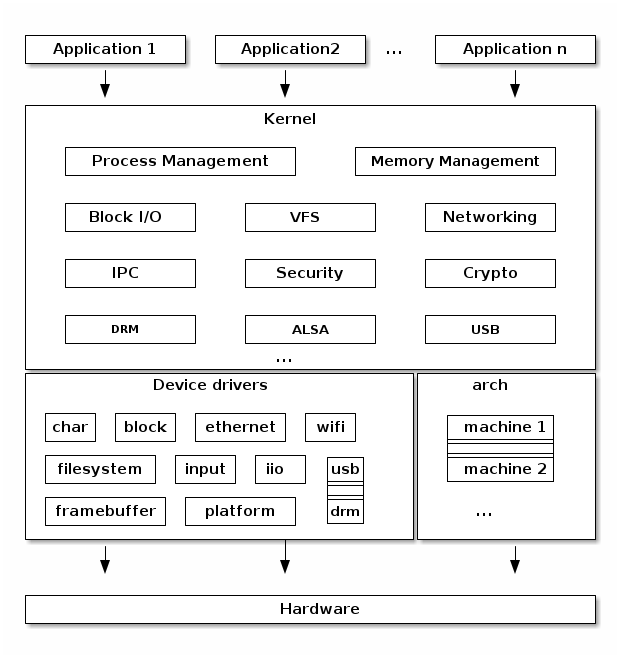
\includegraphics[width=0.85\textwidth]{images_pfe/kernelarchitecture.png}
  \caption{Architecture générale du noyau Linux}
  \label{fig:kernel-arch}
\end{figure}

\begin{description}
  \item[1. Architecture (\texttt{arch})]  
    Contient le code spécifique aux architectures matérielles (x86, ARM, MIPS, PowerPC, IBM S/390, etc.), parfois subdivisé en code machine spécifique.
  \item[2. Pilotes de périphériques (Device Drivers)]  
    Mise en œuvre d’un modèle unifié pour gérer les périphériques : détection, état, bus d’attache et liaison avec le pilote approprié.
  \item[3. Gestion des processus (Process Management)]  
    Création, ordonnancement et terminaison des processus. Implémentation des appels \texttt{fork()}, \texttt{exec()}, \texttt{wait()} et des threads POSIX via la structure \texttt{task\_struct}.
  \item[4. Gestion de la mémoire (Memory Management)]  
    Allocation et libération de la mémoire physique et virtuelle : pagination, swap, \texttt{mmap()}, \texttt{brk()}, allocateurs SLAB et \texttt{vmalloc}.
  \item[5. Gestion du Block I/O (Block I/O Management)]  
    Création et ordonnancement des requêtes d’E/S sur périphériques bloc : RAID logiciel, LVM, fusion et tri des requêtes, planification par ordonnanceurs d’I/O.
\end{description}


\bigskip
L’un des aspects les plus enthousiasmants d’un système d’exploitation moderne — protection, concurrence, virtualisation, allocation de ressources et stockage fiable — est qu’ils se retrouvent aujourd’hui dans de nombreux domaines de l’informatique, au‑delà des seuls noyaux. Il est impossible de concevoir des systèmes informatiques résilients, sécurisés et flexibles sans appliquer ces concepts fondamentaux


\textcolor{blue}{Pour plus d’informations sur larchitecture du noyau linux, consultez \cite{Linux_kernel_course} }  
%\begin{figure}[H]
%  \centering
 % 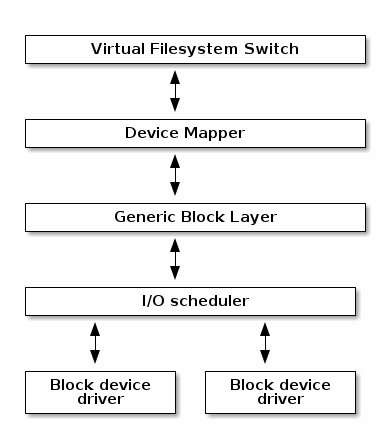
\includegraphics[width=0.85\textwidth]{images_pfe/iomanagmemnt.png}
%  \caption{Architecture du sous‑système Block I/O}
%  \label{fig:io-management}
%\end{figure}
\section{Configuration du noyau}
%\textcolor{red}{TBD: add figure and ressources}
Dans le noyau Linux, il existe deux types de configurations principales :

\begin{enumerate}
  \item \textbf{Intégrée au noyau (built-in)}

  Lorsqu'une option est activée en tant qu’élément intégré (\texttt{built-in}), cela signifie qu’elle est compilée directement dans l’image binaire du noyau (\texttt{vmlinuz}).

  \textbf{Caractéristiques :}
  \begin{itemize}
    \item \textbf{Toujours disponible} : Pas besoin de la charger manuellement, elle fait partie du noyau dès le démarrage.
    \item \textbf{Pas de surcharge à l’exécution} : Exécution plus rapide, car le code est déjà en mémoire.
    \item \textbf{Critique pour le démarrage} : Les pilotes matériels essentiels (ex. : contrôleurs de disque, systèmes de fichiers) doivent être intégrés si nécessaires pendant les premières étapes du démarrage .
  \end{itemize}

  \item \textbf{Modules chargeables (Loadable Kernel Modules)}

  Les fonctionnalités marquées comme \texttt{m} (module) sont compilées séparément sous forme de fichiers objets \texttt{.ko} (Kernel Object), stockés dans \texttt{/lib/modules}.

  \textbf{Caractéristiques :}
  \begin{itemize}
    \item \textbf{Chargés à la demande} : Manuellement via \texttt{modprobe}, ou automatiquement via \texttt{udev}.
    \item \textbf{Utilisation mémoire réduite} : Les modules ne sont chargés que lorsqu’ils sont nécessaires.
    \item \textbf{Flexibilité de mise à jour} : Les modules peuvent être recompilés ou rechargés sans nécessiter de redémarrage du système.
  \end{itemize}
\end{enumerate}




Pour \textsc{Kraken OS}, nous avons retenu le noyau Linux \texttt{6.10.5}, garantissant un équilibre entre stabilité et fonctionnalités récentes. Nous avons activé uniquement les modules nécessaires aux architecture cible  x86\_64, et désactivé les options optionnelles afin de réduire l’empreinte mémoire et d’optimiser les performances. 


\section{Systèmes d'initialisation : System V et SystemD}
\label{sssec:sysv}

Il existe deux principaux types de systèmes d'initialisation : \textbf{SystemD} et \textbf{System V}. \\
System V est plus ancien. Il s'appuie sur un petit programme appelé \texttt{init}, dont le rôle est de configurer les processus de base du système et d'exécuter un script principal (nommé \texttt{rc}). Ce script orchestre une série de scripts secondaires destinés à initialiser les services système.

SystemD est un système plus moderne, conçu pour permettre \textbf{un démarrage plus rapide} et une \textbf{meilleure gestion des dépendances}.

\begin{itemize}
    \item \textbf{SystemD} utilise des fichiers \texttt{.service} pour contrôler les processus.
    \item \textbf{System V} repose sur des scripts shell situés dans \texttt{/etc/init}.
\end{itemize}

\bigbreak
Il est clair que SystemD est plus moderne et adopté par la majorité des distributions récentes. Toutefois, il est également \textbf{plus complexe}, notamment dans sa \textbf{gestion des dépendances}. \\
C’est pourquoi nous avons choisi d’utiliser System V — tout simplement pour sa simplicité — car, à ce stade, notre objectif principal était d’obtenir un système bootable.

Nous ignorions alors que ce choix constituerait une \textbf{erreur stratégique}, car il a engendré plusieurs inconvénients :
\begin{itemize}
    \item un temps de démarrage plus long,
    \item un traitement séquentiel des services,
    \item une complexité accrue lors de l’ajout de nouveaux scripts.
\end{itemize}

Nous travaillerons dur dans la prochaine version de la distribution pour résoudre ce problème en utilisant SystemD à la place de System V.

%\begin{itemize}
 %   \item \textbf{Temps de démarrage allongé} : Une instance basique de notre système démarre en 8 à 12 secondes (mesurées du premier message du noyau jusqu'à l'invite de connexion).
    
  %  \item \textbf{Traitement séquentiel} : Un retard dans un processus  bloque l'ensemble du démarrage.
    
   % \item \textbf{Complexité d'ajout} : L'ajout de nouveaux services nécessite une planification manuelle de l'ordre d'exécution.
%\end{itemize}

\textcolor{blue}{Pour une analyse détaillée de SystemD vs System V, voir \cite{systemV_systemD}.}


\section{Qu'est-ce qu'un bootloader ?}

Il existe deux grands chargeurs d'amorçage (bootloaders) pour les systèmes Unix : \textbf{GRUB} et \textbf{Syslinux}.  \\
Dans \textsc{Kraken OS}, nous avons choisi d’utiliser \textbf{GRUB} pour démarrer le système depuis le disque, et \textbf{Syslinux} pour l’intégration dans le fichier ISO bootable.  

%Nous parlerons de \textbf{Syslinux} dans les chapitres suivants, mais concentrons-nous maintenant sur \textbf{GRUB}.



\medskip
\noindent
En bref, un \textit{bootloader} est le premier programme logiciel exécuté au démarrage d’un ordinateur. Il est responsable du chargement et du \textbf{transfert de contrôle} vers le noyau du système d’exploitation.  
Ce dernier se charge ensuite de l’initialisation complète du système.

Pour visualiser ce processus, reportez-vous à la figure suivante qui montre un schéma simplifié du démarrage :

\begin{figure}[H]
  \centering
  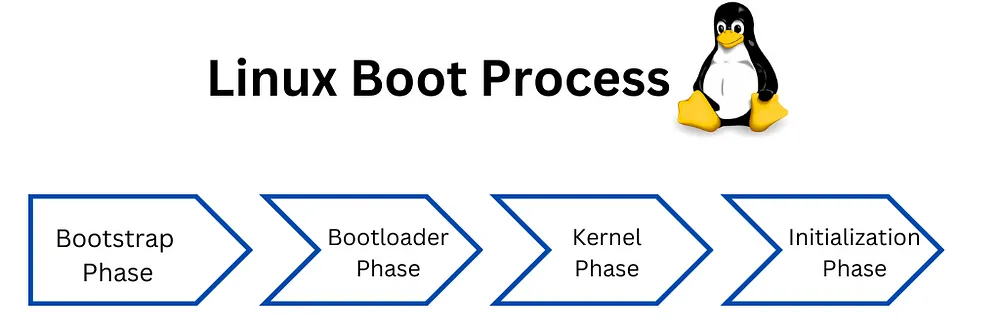
\includegraphics[width=0.85\textwidth]{images_pfe/simplebootprocess.png}
  \caption{Processus de démarrage simplifié}
  \label{fig:botprocess}
\end{figure}



\bigskip
\noindent
GRUB adopte une syntaxe particulière pour désigner les disques et leurs partitions.  
Cette notation suit le format \texttt{(hdX,Y)}, où :
\begin{itemize}
  \item \texttt{X:} représente le numéro du disque dur
  \item \texttt{Y:} désigne le numéro de la partition
\end{itemize}

\noindent
Par exemple :

\begin{table}[h!]
    \centering
    \begin{tabular}{|l|l|}
    \hline
    \textbf{Disque physique} & \textbf{Notation GRUB} \\
    \hline
    \texttt{/dev/sda1} & \texttt{(hd0,1)} \\
    \texttt{/dev/sdb3} & \texttt{(hd1,3)}\\
    
    \hline
    \end{tabular}
    \caption{Correspondance des partitions selon GRUB}
    \label{tab:grub-part}
\end{table}
\clearpage
 GRUB comprend plusieurs utilitaires tels que \texttt{grub-install}, \texttt{grub-mkfont} et \texttt{grub-mkconfig}.

\begin{enumerate}
  \item \textbf{\texttt{grub-install}} est l’outil principal : il accepte comme argument un disque (par exemple \texttt{/dev/sda}), détecte automatiquement la partition marquée comme amorçable et installe GRUB sur le disque souhaité.
  \item \textbf{\texttt{grub-mkfont}} génère des polices qui pourront ensuite être utilisées dans la configuration du thème GRUB.
  \item \textbf{\texttt{grub-mkconfig}} permet de créer automatiquement le fichier de configuration \texttt{grub.cfg}. \\
 
  \textbf{Remarque} :Sur notre distribution, cette opération "grub-mkconfig" échoue souvent car elle dépend de configurations RAID, LVM, etc. Il est donc nécessaire de creer  manuellement notre propre fichier \texttt{grub.cfg}.
\end{enumerate}


\textcolor{blue}{Pour plus de detaille , voir \cite{grub_doc}.}


\section{Conclution}
Le noyau Linux, les scripts de démarrage SystemV et le chargeur d’amorçage (bootloader) fonctionnent de manière interdépendante pour amorcer le système.  Une simple pression sur le bouton d’alimentation déclenche une cascade d’étapes 

Le signal électrique initialise le BIOS/UEFI , Le chargeur d’amorçage (GRUB)  lit grub.cfg pour charger le noyau et le initrd,Le noyau monte le système de fichiers racine (rootfs) et lance /sbin/init,
Les scripts SystemV initialisent les services pour aboutir à votre environnement de travail final.\\


\clearpage